\documentclass[border=4pt]{standalone}
\usepackage{tikz}
\usepackage{pgfplots}
\pgfplotsset{compat=1.17}
\usepackage[table]{xcolor}
\usetikzlibrary{shapes.geometric, arrows.meta, positioning, fit, calc}
\definecolor{headingblue}{HTML}{1F4E79}
\definecolor{lightblue}{HTML}{D9EAF7}
\definecolor{softgray}{HTML}{F4F6F8}
\definecolor{darkgray}{HTML}{404040}
\definecolor{prismagreen}{HTML}{E8F5E9}
\definecolor{prismabox}{HTML}{1565C0}
\definecolor{chartblue}{HTML}{2196F3}
\definecolor{chartorange}{HTML}{FF9800}
\definecolor{chartgreen}{HTML}{4CAF50}
\definecolor{chartred}{HTML}{F44336}
\definecolor{chartpurple}{HTML}{9C27B0}
\definecolor{chartgray}{HTML}{9E9E9E}
\begin{document}
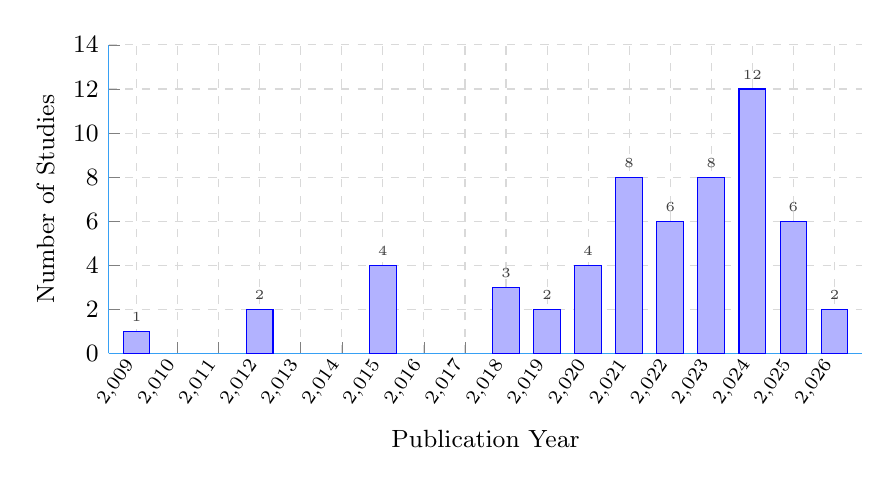
\begin{tikzpicture}
\begin{axis}[
  ybar,
  bar width=0.34cm,
  width=0.92\textwidth,
  height=5.5cm,
  xlabel={Publication Year},
  ylabel={Number of Studies},
  xtick={2009,2010,2011,2012,2013,2014,2015,2016,2017,2018,2019,2020,2021,2022,2023,2024,2025,2026},
  xticklabel style={rotate=55, anchor=east, font=\scriptsize},
  yticklabel style={font=\small},
  xlabel style={font=\small},
  ylabel style={font=\small},
  ymin=0, ymax=14,
  ytick={0,2,4,6,8,10,12,14},
  nodes near coords,
  nodes near coords style={font=\tiny, color=darkgray},
  axis lines*=left,
  enlarge x limits=0.04,
  fill=chartblue!70,
  draw=chartblue!90,
  tick align=inside,
  grid=major,
  grid style={dashed, gray!30},
]
\addplot coordinates {
  (2009,1) (2012,2) (2015,4) (2018,3) (2019,2) (2020,4) (2021,8) (2022,6) (2023,8) (2024,12) (2025,6) (2026,2)
};
\end{axis}
\end{tikzpicture}
\end{document}
